\section{Video Input}
This section describes the effort that was put into getting camera input for the system (functional requirement FR3).
Throughout the working period the approach to this was changed multiple times as we learned more about the hardware we were working with.

\subsection{Raspberry Pi Camera}
After some consideration it was decided that the \textit{Raspberry Pi Camera Board}\footnote{\url{https://www.raspberrypi.org/products/camera-module/}} (PiCamera) would be used as the camera module for the system.
The circumstances leading to this choice are discussed in Section \ref{sec:camera_discussion}.

\begin{figure}[h]
    \centering
    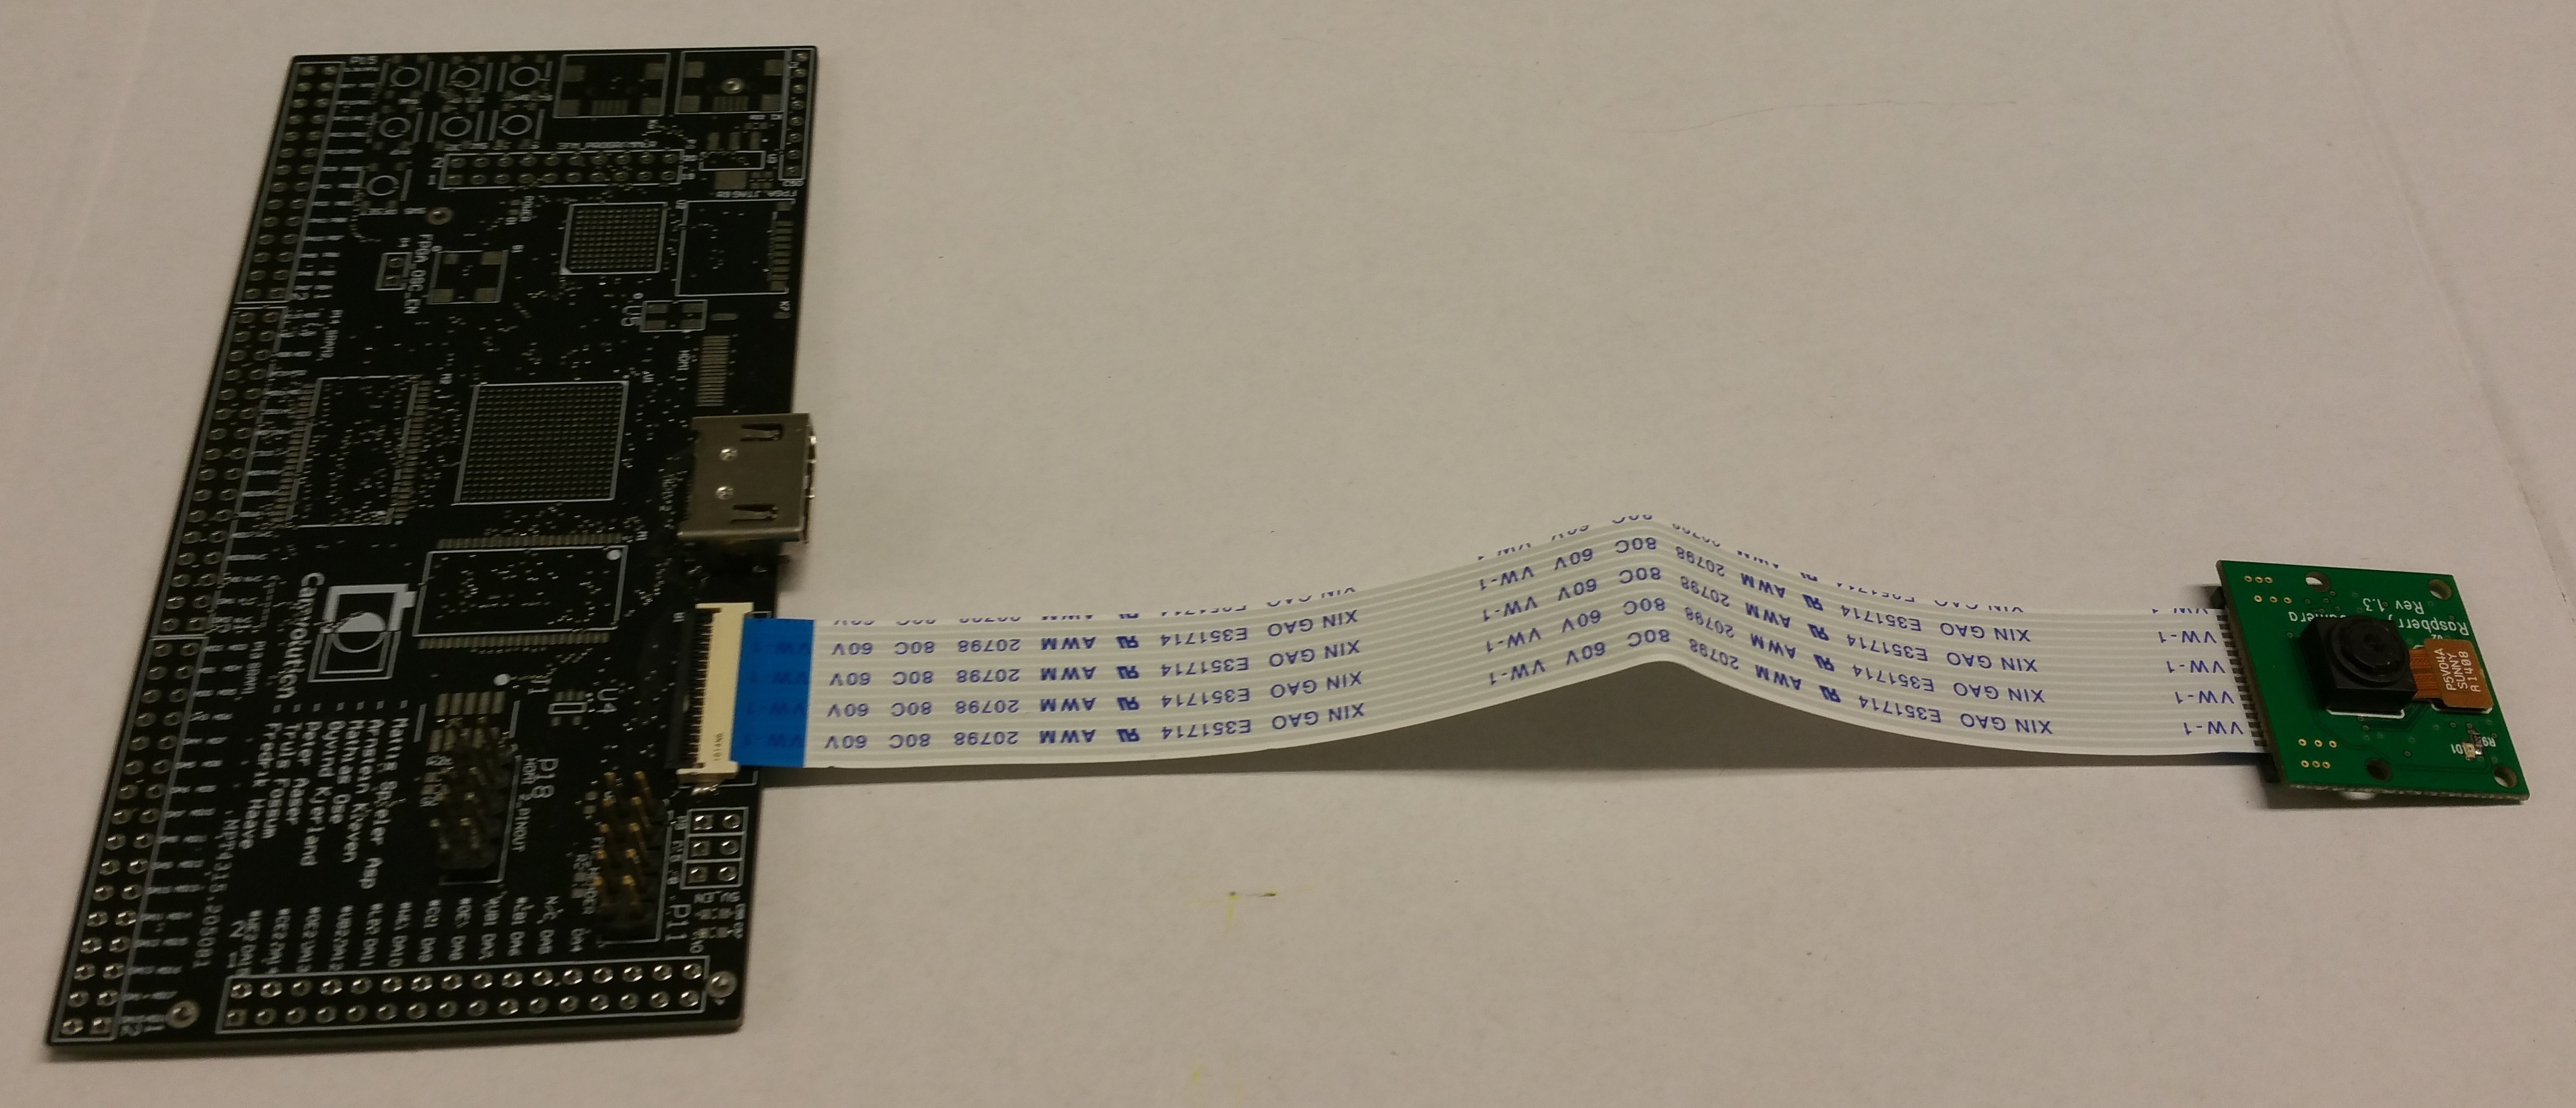
\includegraphics[width=0.75\textwidth]{img/picamera}
    \caption{Raspberry Pi Camera connected to Camvolution board}
\end{figure}

The \textit{Raspberry Pi Foundation} has designed this peripheral for use with the \textit{Raspberry Pi} computer.
The PiCamera can take still shots as well as record continuous video.
The module consists of a camera sensor on a board with a controller unit which connects to the Pi (or another master device) via a 16-pin ribbon cable.
Communication over this cable is defined by the proprietary \textit{MIPI Camera Serial Interface} (CSI) specification.

The master device controls the camera module by sending instructions over an I2C bus on the ribbon cable,
and the camera module responds with picture data over two clocked differential busses.\cite{picam-pinout}
Parameters that may be controlled include video encoding, resolution in two dimensions and framerate.


\subsection{SD Card Video}
One possible source of video is a file stored on the SD card connected to the board.
The MCU is able to open files and pass the data from it to the processor over EBI.
For simplicity of development the MCU should not need to handle encoded video. Instead, the video files should contain raw pixel data so that it can easily be streamed to the processor.


\subsection{Options for Video Path}
\begin{figure}
    \centering
    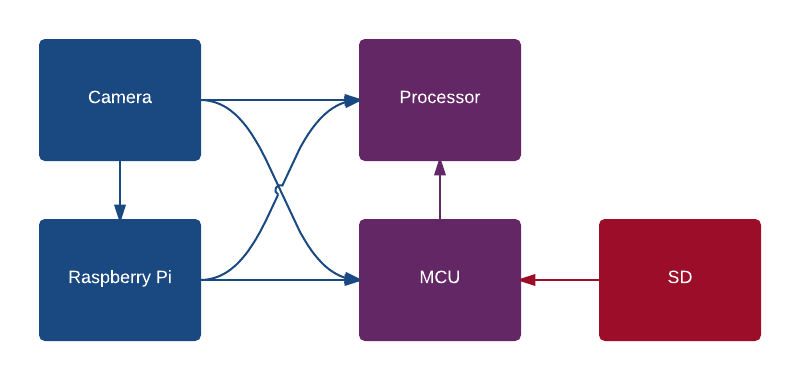
\includegraphics[width=\linewidth]{img/VideoPath}
    \caption{Paths an input video stream could take to reach the processor.}
    \label{fig:VideoPath}
\end{figure}

Because the group had no experience with video input,
there was a lot of uncertainty of how to transfer video from the camera to the processor.
What we decided we wanted to do was to have both video camera and data from SD card as possible sources,
with the possibility to switch between them by using the buttons on the board.
Figure \ref{fig:VideoPath} shows an overview of the possible paths a video stream could take from camera,
and some options that were explored are briefly outlined below:

\begin{description}
    \item[PiCamera Connected to Board, Controlled by MCU]
        \hfill\\
        Wiring the camera connector to the MCU, having software on the MCU control the camera and receive the video stream before forwarding it to the FPGA.
    \item[PiCamera Connected to Board, Controlled by FPGA]
        \hfill\\
        Wiring the camera connector directly to the FPGA, having a FPGA submodule control the camera and receive the video stream.
    \item[PiCamera Connected to Raspberry Pi, Transfer Over With Bus]
        \hfill\\
        Having the Raspberry Pi control the camera using the provided libraries.
        Transfer video stream to Camvolution using a parallel bus controlled by GPIO software.
    \item[PiCamera Connected to Raspberry Pi, Transfer With SPI]
        \hfill\\
        Having the Raspberry Pi control the camera using the provided libraries.
        Transfer the video stream to Camvolution using built-in SPI hardware.
    \item[SD Card Video]
        \hfill\\
        Instead of using the camera, have a recorded video stored on the SD card which the MCU can forward to the FPGA.
    \item[HDMI Input]
        \hfill\\
        Instead of using the camera, use the second HDMI port on the board for input from any HDMI source.
\end{description}

\subsection{Reverse-Engineering the Camera Control Protocol}
\begin{figure}
    \centering
    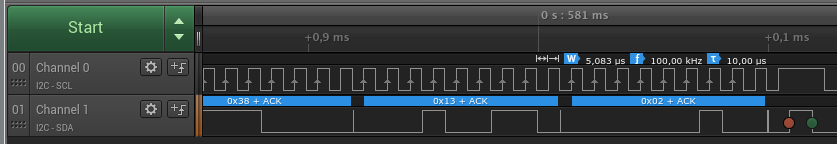
\includegraphics[width=\linewidth]{img/logic/pi_cam_i2c}
    \caption{I2C communication between Raspbery Pi and PiCamera}
    \label{fig:PiCamI2C}
\end{figure}

The Raspberry Pi controls the PiCamera by sending signals over a two-wire serial bus (I2C).
At the beginning of the project we wrongly assumed that there would be adequate documentation of this control protocol.
As this didn't work out, an attempt was made to use a logic analyzer to "listen in" on the communication between the Raspberry Pi and PiCamera.
A screenshot of this can be seen in Figure \ref{fig:PiCamI2C}.

\subsection{MCU as Camera Controller}
\begin{figure}
    \centering
    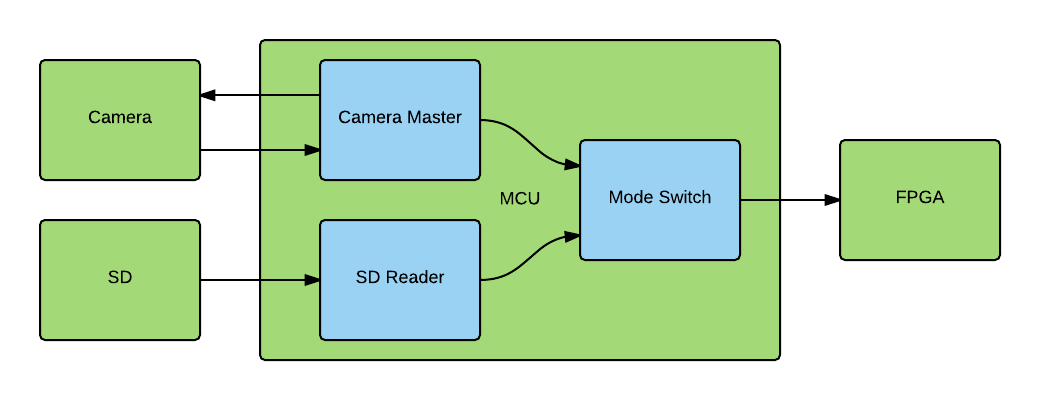
\includegraphics[width=\linewidth]{img/MCU_CameraMaster}
    \caption{MCU as input controller. Hardware components in green, software components in blue.}
    \label{fig:MCU_CameraMaster}
\end{figure}

The first option explored was to have the MCU be the camera controller and receive the video stream.
This idea was abandoned eventually as the EFM32GG does not have hardware to receive the differential bus data,
so the FPGA would be more appropriate for this role.

\subsection{FPGA as Camera Controller}
\begin{figure}
    \centering
    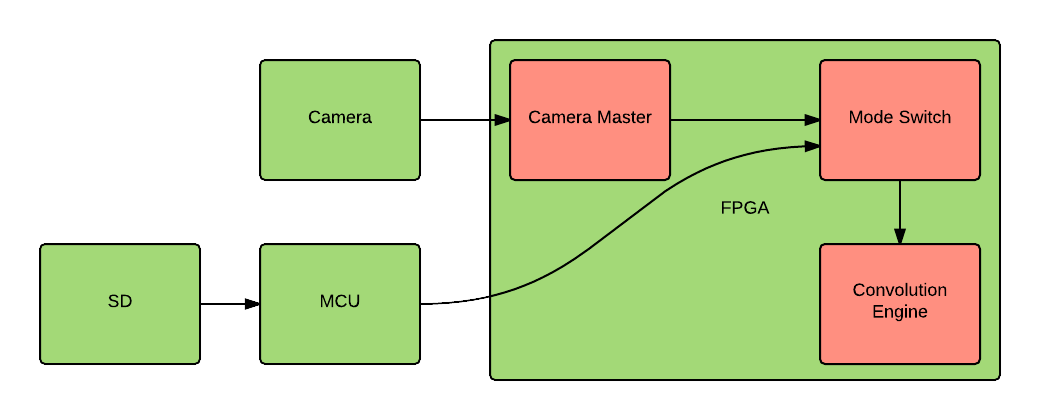
\includegraphics[width=\linewidth]{img/FPGA_CameraMaster}
    \caption{FPGA with input controller module. Hardware components in green, FPGA submodules in red.}
    \label{fig:FPGA_CameraMaster}
\end{figure}

With a snapshot of the I2C communication procured,
a VHDL module was written that could output the same sequence,
and this was tested with the Spartan-6 development board and the PiCamera.
While the FPGA was able to output the I2C sequence,
the camera would not send acknowledgements for any of the transmissions.
Efforts into figuring out why the PiCamera wouldn't respond were fruitless, so the idea was eventually abandoned.

\subsubsection{Using the Raspberry Pi}
An option to reverse-engineering the camera control protocol was to use a Raspberry Pi to control the camera,
then transfer the video stream to the Camvolution board.
The provided software on the Pi makes it very easy to have full control of the camera,
but transferring video out of the Pi at high rates is more challenging.

\subsubsection{GPIO Pins}
The Raspberry Pi has GPIO pins that are controllable in software.
A script was written which could output pixel data to the GPIO pins as a parallel bus with one clock pin and 8 data pins.
This was very simple to implement, however it was also very slow.
With a Raspberry Pi 2 the best clock frequency achieved was ca. $600kHz$.
This would only allow sending very small frames of video at low framerates,
so the idea was put on hold and other options explored.

The Raspberry Pi also has hardware support for SPI over some of the GPIO pins.
Directing the video stream to this instead was more promising,
since the frequency of the clock in this mode was able to go up to a $32MHz$\footnote{\url{http://elinux.org/index.php?title=RPi\_SPI\#Speed\_2}},
which would be a massive improvement even if the transfer was serial instead of 8-bit parallel.
Unfortunately what was observed was that while the transfer of chunks of data was fast,
there were long delays between chunks.
At 240x240 resolution, 6 frames per second was the best transfer rate that was able to keep up with the recording.
Figures \ref{fig:Logic7fps} and \ref{fig:Logic1Frame} shows the logic analyzer output for SPI transfers.

\begin{figure}
    \centering
    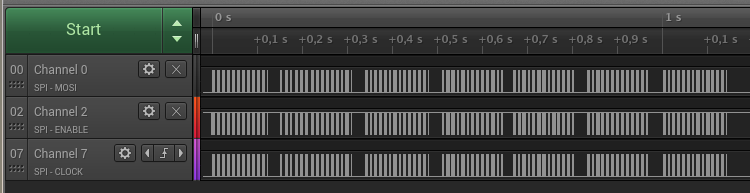
\includegraphics[width=\linewidth]{img/logic/7fps}
    \caption{At 7 FPS recorded, the SPI transmission is unable to keep up and sends the seventh frame too late.}
    \label{fig:Logic7fps}
\end{figure}

\begin{figure}
    \centering
    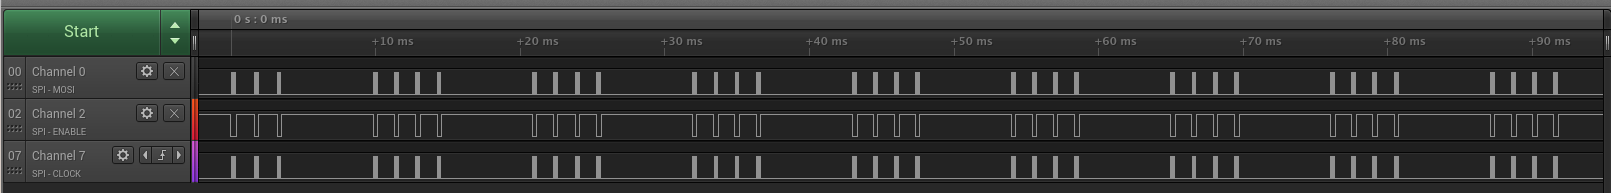
\includegraphics[width=\linewidth]{img/logic/1frame}
    \caption{Inspecting a single frame transmission closer reveals a lot of idle time.}
    \label{fig:Logic1Frame}
\end{figure}

\subsubsection{HDMI Output}
Seeing that all efforts into using the camera were either failing or at best offering a tiny stream of data,
we decided to concentrate on the HDMI input of the Camvolution system.
The Raspberry Pi has HDMI out, so it would definently be possible to use the PiCamera with this setup.

